%\label{Replicating_Existing_Rainfall_Model}

In this chapter, we will explore existing rainfall models, with a particular focus on HMMs. We will replicate results found using HMMs and discuss potential drawbacks.

\section{Cowpertwait}
\label{Replicating_Existing_Rainfall_Model:Cowpertwait}
Cowpertwait's rainfall models have been used for decades with a good deal of success. This section will aim to explain the motivations behind Cowpertwaits models.

Although we will not dive deep into his methodology, one may reference the following paper for more information. All papers are available in the bibliography. The earliest paper we have referenced is \cite{Cowpertwait1994}.

Over time, Cowperthwait has improved and adjusted his model for varying applications. For example, in one of his more recent papers \cite{Cowpertwait2010}, Coppertwait has turned the discrete variable describing the type of storm into a continuous one. These changes and developments, while interesting, are not the focus of our paper. Instead, we will focus on \cite{Cowpertwait1994} to understand the model at its simplicity, and one may apply these ideas to a Hidden Markov Model. 

All of Cowpertwaits models use Neyman-Scott point processes to describe the arrival of Storms. The model itself is as follows:
\begin{itemize}
    \item The origin of each storm is a Poisson process in space-time
    \item Each storm is a circular region in two-dimensional space with radii given by independent exponential random variables.
    \item Each storm generates a cluster of two-dimensional circular rain cells with random duration, position and radius. 
    \item The duration of each cell is an exponential random variable.
    \item The intensity of each cell is a random exponential distributed but dependent on the cell type. In \cite{Cowpertwait1994} we have two cell types, light and heavy.
    \item Overall intensity at any point is given by the sum of overlapping intensities at the point in space and time.
\end{itemize}

The GNSRP Model is a generalisation of the Neyman-Scott-Rectangular-Pulse (NSRP) Model with only one cell type. The key feature of the NSRP is that, in addition to those above, the distance from Cell origins to its Storm origin are independently exponentially distributed. Unlike other models that used an independent uniform distribution for this, NSRP accounted for the realistic effect that rainfall tends to be more intense near the storm's centre.

\section{Grando}
\label{Replicating_Existing_Rainfall_Model:Grando}
Grando extended on Cwppertwait's ideas in \cite{Grando2019}. She completely removes the double-disc structure and attempts to enclose the correlations within the larger Storm discs from Cowpertwait in the Hidden Markov States. In this section, we will explore her model and how she fits her parameters.

    \subsection{Model}
    \label{Replicating_Existing_Rainfall_Model:Grando:Model}
    This subsection presents Grando's Rainfall Model in a summariesed way.

    Grando defines her discrete time intensity process as follows:
    For $n \geq 1$ and $x \in A$, where $A \subset \mathbb{R}^2$
    \begin{equation}
        I_n(x) := \sum_{i=1}^{N^{(n)}} \sigma_i^{(n)} \mathbb{I}_{D(x_i^{(n)},R_i^{(n)})} (x)
    \end{equation}
    where:
    \begin{itemize}
        \item $I_n(x)$ is the rain intensity
        \item $N^{(n)} \sim$ Pois($\lambda$) represents the number of rain discs generated
        \item $\sigma_i^{(n)} \sim$ Exp($\tau$) is a random variable providing the rain intensity
        \item  $D(x_i^{(n)},R_i^{(n)})$ is a rain disc with centre $x_i^{(n)} \sim$ Unif($A$) and radius $R_i^{(n)} \sim$ Exp($\xi$).
        \item $\mathbb{I}_{D(x_i^{(n)},R_i^{(n)})} (x)$ is an indicator function, equal to 1 if the current rain disc overlaps position $x$.
    \end{itemize}

    Parameters $\lambda$,$\xi$ and $\tau$ are taken to be fixed for each type of storm. In other words, for each hidden state of the HMM, there is a unique $\lambda$,$\xi$ and $\tau$. Informally, the model has hidden states which determine the type of storm. This then dictates the values of the three above parameters, which influences the intensity of rain observed.

    Thus we arrive at the learning problem. Due to the added complexity of additional parameters, we cannot directly use methods for HMMs discussed earlier in the paper. Direct likelihood calculation is complex for HMMs alone; after introducing these additional parameters, it is not feasible. 

    Given the model has $m$ states, we will have $m^2+4m$ unknown parameters, $m^2$ for the transition probabilities, $m$ for the initial distribution and $m$ for each of $\lambda$,$\xi$ and $\tau$.  This problem is high-dimensional. To overcome this, Grando fixes certain parameters in order to gain a better understanding of the remaining. She uses two methods; Nelder-Mead and Approximate Bayesian Computation \ref{Model_Selection:Approximate_Bayesian_Computation}. We will focus on the latter as it has provided superior results in her testing.

    \subsection{Fitting}
    \label{Replicating_Existing_Rainfall_Model:Grando:Fitting}

    In this subsection, we will explore Grando's Model's fitting methodology. 

    We begin by trying to replicate Grando's results in order to establish a starting point. For ABC, we require the prior distribution along with a summary statistic. Deriving the prior distribution is not a trivial problem. We have parameters for the HMM and parameters for the observations but have to extract both from only the rainfall intensity data. 

    Grando determines that even without the HMM parameters, the problem is high dimensional (3$m$ parameters). She decides to fix all HMM parameters to uniform(0,1) for each test whilst ensuring the transition matrix is stochastic through the normalisation of rows. She believes that this will allow her to retrieve close approximations of all $\lambda$,$\xi$ and $\tau$ from the data, which she can then use to calculate the HMM parameters. 

    For each simulation, she will generate a new value for all $\lambda$,$\xi$ and $\tau$. Then plot the summary statistic against the values for each and then find areas of high concentration to decide what a suitable approximation for the actual value of each is. Here, she sets her ABC tolerance to $\infty$ and then manually narrows her range through the graph.

    Grando picks values for each parameter using the uniform distribution between preset values. She says, "This technique is purely heuristic, and only aimed to explore the problem, as decisions made are completely arbitrary.". Theoretically, we could pick any values, but we will match the values she has used for consistency.  

    She decides to use the mean intensity as her summary statistic for ABC. She calculates this for both the simulated and given data. She then calculates the normalised Euclidean distance between the two as her metric for model performance.


\section{Replicating Grando}
\label{Replicating_Existing_Rainfall_Model:Replicating_Grando}
This section will be replicating Grando's results to analyse her finding in further depth and explore the following stages for research. We replicate both nine-parameter and three-parameter estimation, in addition to our improved algorithm used to test the validity of the testing methodology itself.

We will be using the same algorithm, same data and same parameters as Grando to ensure consistency. Our data measures rainfall across 30 sites in Germany over the period from 1st January 1931 to 31st December 2000. Co-ordinate data for each site is also given in an additional file, labelled as Easting and Northing. 

Grando fixes $m$=3, allowing for a low, medium and high state for rainfall. This gives us 21 unknown parameters, of which we are attempting to estimate 9.

All programs have been run on the personal desktop (AMD Ryzen™ 9 3900X with 12 Cores and 24 Threads running from 3.8GHz up to 4.6GHz) using C++20.


    \subsection{Code}
    \label{Replicating_Existing_Rainfall_Model:Replicating_Grando:Code}
    We present a brief summary of the coding process in this subsectino.

    To ensure the validity of the results, we wanted to run multiple tests. Grando's code was written in R and required multiple hours to produce a result. To improve on this, we have rewritten the program in C++ and used Python on Jupyter Notebooks for analysis.

    Data preparation took place in excel. For simplicity in importing into C++, the data needed to be configured in a particular way. This configuration is described thoroughly in the notes given with the code. 

    C++ was used for the actual simulation as this was the slowest part of Grando's algorithm. Many parameters have been hardcoded. This is to allow for efficiency and can later be altered if needed. The code has been Multi-threaded for further reduction in run-time. Admittedly the code can be further parallelised, but in its current state, it is acceptable; run times of under 5 minutes. 

    Analysis was done using Python in Jupyter Notebooks. The C++ program created multiple CSV files as output, and these were taken as input for analysis. 

    \subsection{Results}
    \label{Replicating_Existing_Rainfall_Model:Replicating_Grando:Results}
    In this subsection, we present our results when replicating Grando's work in \cite{Grando2019}. We finish with our adjusted test to show why Grando's estimation methodology was flawed.

        \subsubsection{Nine Parameter Estimation}
        \label{Replicating_Existing_Rainfall_Model:Replicating_Grando:Results:Nine_Parameter_Estimation}

        We begin with using ABC to estimate all parameters, found on pages \cite{Grando2019}[75-76]. The parameters are picked as follows:

        \begin{itemize}
            \item $\lambda_1 \sim \text{Unif(5,15)}$, $\lambda_2 \sim \text{Unif(16,25)}$ and $\lambda_3 \sim \text{Unif(26,35)}$
            \item $\xi_1 \sim \text{Unif(0.03,0.07)}$, $\xi_2 \sim \text{Unif(0.008,0.02)}$ and $\xi_3 \sim \text{Unif(0.001,0.007)}$
            \item $\tau_1 \sim \text{Unif(0.8,1.4)}$, $\tau_2 \sim \text{Unif(0.3,0.7)}$ and $\tau_3 \sim \text{Unif(0.07,0.2)}$
        \end{itemize}

        For each simulation, we generate data for 365x5 days and calculate the normalised Euclidean distance between the mean and mean of the whole given dataset. Due to random sampling, we attempt to find estimates for all nine parameters simultaneously. We completed 200 iterations on the personal desktop in 42.2841 seconds.


        \begin{figure}
            \centering
            \begin{subfigure}{.3\textwidth}
                \centering
                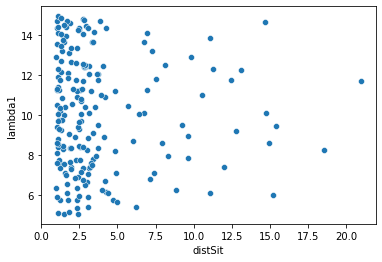
\includegraphics[width=\linewidth]{./AllParam/lambda_1.png}
                \caption{$\lambda_1$ }
                \label{allp:lambda1}
            \end{subfigure}
            \begin{subfigure}{.3\textwidth}
                \centering
                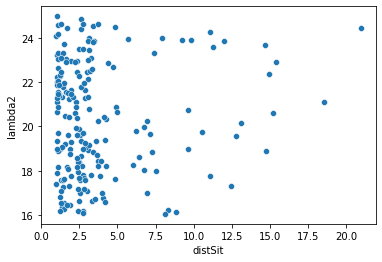
\includegraphics[width=\linewidth]{./AllParam/lambda_2.png}
                \caption{$\lambda_2$ }
                \label{allp:lambda2}
            \end{subfigure}    
            \begin{subfigure}{.3\textwidth}
                \centering
                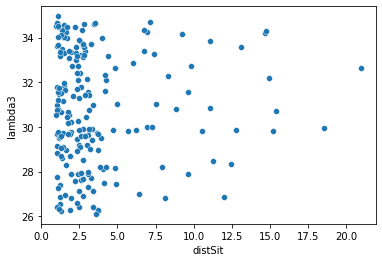
\includegraphics[width=\linewidth]{./AllParam/lambda_3.png}
                \caption{$\lambda_3$ }
                \label{allp:lambda3}
            \end{subfigure}
            \begin{subfigure}{.3\textwidth} 
                \centering
                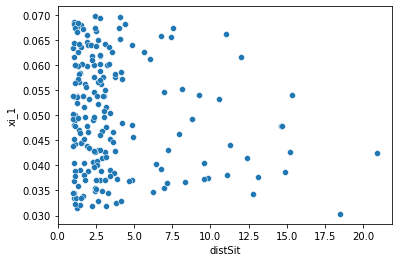
\includegraphics[width=\linewidth]{./AllParam/xi_1.png}
                \caption{$\xi_1$ }
                \label{allp:xi1}
            \end{subfigure}
            \begin{subfigure}{.3\textwidth}
                \centering
                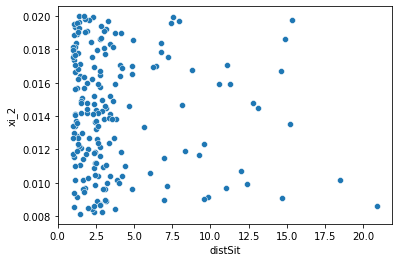
\includegraphics[width=\linewidth]{./AllParam/xi_2.png}
                \caption{$\xi_2$ }
                \label{allp:xi2}
            \end{subfigure}
            \begin{subfigure}{.3\textwidth}
                \centering
                \includegraphics[width=\linewidth]{./AllParam/xi_3.png}
                \caption{$\xi_3$ }
                \label{allp:xi3}
            \end{subfigure}
            \begin{subfigure}{.3\textwidth}
                \centering
                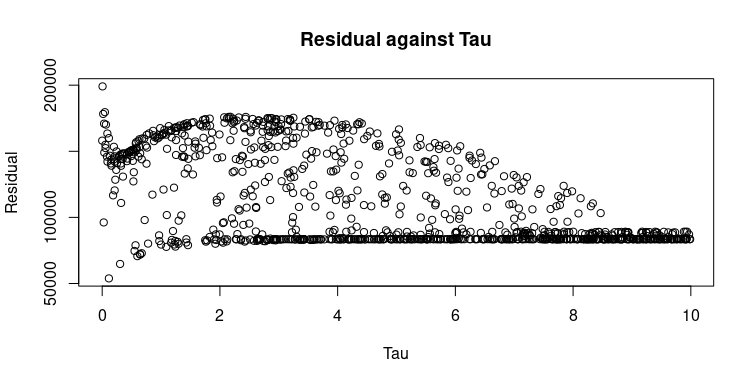
\includegraphics[width=\linewidth]{./AllParam/tau_1.png}
                \caption{$\tau_1$ }
                \label{allp:tau1}
            \end{subfigure}
            \begin{subfigure}{.3\textwidth}  
                \centering
                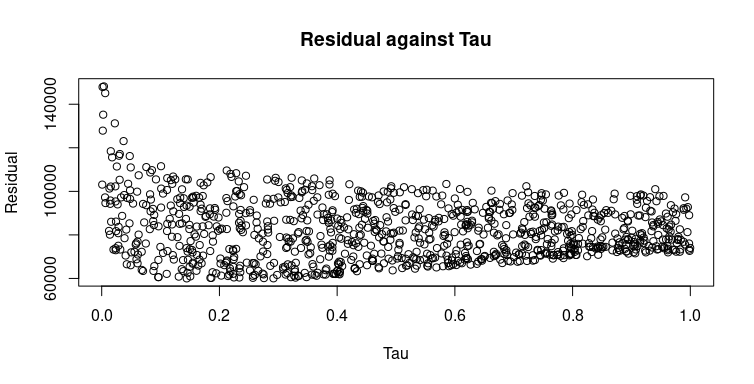
\includegraphics[width=\linewidth]{./AllParam/tau_2.png}
                \caption{$\tau_2$ }
                \label{allp:tau2}
            \end{subfigure}
            \begin{subfigure}{.3\textwidth}
                \centering
                \includegraphics[width=\linewidth]{./AllParam/tau_3.png}
                \caption{$\tau_3$ }
                \label{allp:tau3}
            \end{subfigure}

            \caption{Parameter values plotted against corresponding normalised Euclidean Distance between simulation and data means.}
            \label{allp}
        \end{figure}
            
        The results show ABC on nine parameters was not successful. Figure \ref{allp} shows an extremely uniform scatter for all parameters suggesting the posterior distribution is still uniform in a neighbourhood of the actual parameters. These results are an exact match to Grando's. 



        \subsubsection{Three Parameter Estimation}
        \label{Replicating_Existing_Rainfall_Model:Replicating_Grando:Results:Three_Parameter_Estimation}
        
        Grando then decides to perform ABC on a subset of our nine parameters. She claims choosing only  $\lambda_i$, only $\xi_i$ or only $\tau_i$ does not yield better outcomes. She then tests for only $\lambda_3$,$\xi_3$ and $\tau_3$, fixing all other parameters to arbitrary values. Once again, for consistency, we choose values to match those of Grando.

        \begin{itemize}
            \item $\lambda_1 = 10$, $\lambda_2 = 20$ and $\lambda_3 =30$
            \item $\xi_1 = 0.05$, $\xi_2 = 0.01 $ and $\lambda_3 =0.005$
            \item $\tau_1 =1.1$, $\tau_2 = 0.5$ and $\tau_3 =0.1$
        \end{itemize}

        For each test we require three simulations. When computing for $\lambda_3$ we change its value from 30 to $\lambda_3 \sim \text{Unif(26,35)}$. Similarly, when computing for $\xi_3$, we change its value to $\xi_3 \sim \text{Unif(0.001,0.007)}$ and when computing for $\tau_3$ we change its value to $\tau_3 \sim \text{Unif(0.07,0.2)}$. At any given time there is one random variable between our nine that we are testing. For efficiency we process this over multiple threads. We completed 100 iterations and ran 5 attempts on the personal desktop. Attempt time ranged between 152.725 in to 199.386 seconds.

        The graphs found in Figures \ref{singlelam}, \ref{singlexi} and \ref{singletau} correspond to the ones found in Grando’s *** REF** paper pages 78-80. We have come across unexpected results. Although the graphs show a similar pattern, there is an inconsistency in values. 


        \begin{figure}
            \begin{subfigure}{.3\textwidth}
            \centering
            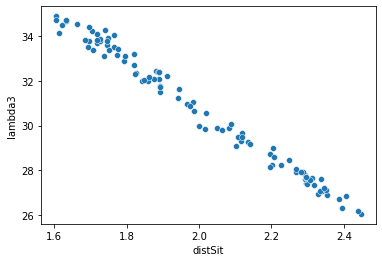
\includegraphics[width=\linewidth]{./SingleParam/lambda_3_1.png}
            \caption{Attempt 1}
            \label{singlelam:1}
            \end{subfigure}
            \begin{subfigure}{.3\textwidth}
            \centering
            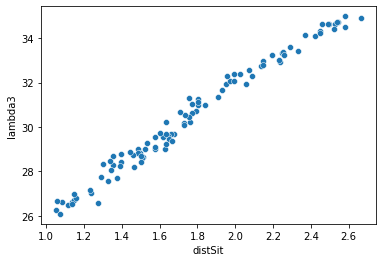
\includegraphics[width=\linewidth]{./SingleParam/lambda_3_2.png}
            \caption{Attempt 2}
            \label{singlelam:2}
            \end{subfigure}
            \begin{subfigure}{.3\textwidth}
                \centering
                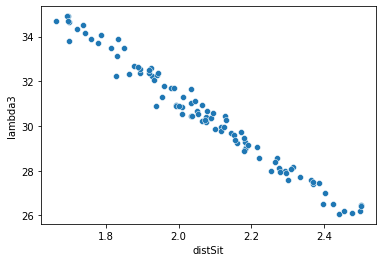
\includegraphics[width=\linewidth]{./SingleParam/lambda_3_3.png}
                \caption{Attempt 3}
                \label{singlelam:3}
            \end{subfigure}

            \centering
            \begin{subfigure}{.3\textwidth} 
                \centering
                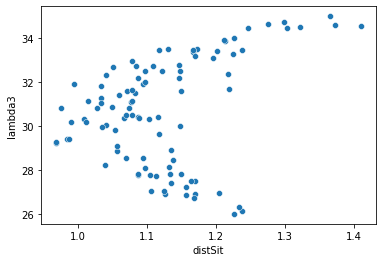
\includegraphics[width=\linewidth]{./SingleParam/lambda_3_4.png}
                \caption{Attempt 4}
                \label{singlelam:4}
            \end{subfigure}
            \begin{subfigure}{.3\textwidth}
                \centering
                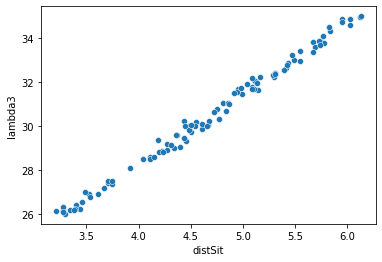
\includegraphics[width=\linewidth]{./SingleParam/lambda_3_5.png}
                \caption{Attempt 5}
                \label{singlelam:5}
            \end{subfigure}

            \caption{$\lambda_3$ values plotted against corresponding normalised Euclidean Distance between simulation and data means for 5 attempts.}
            \label{singlelam}
        \end{figure}

        For $\lambda_3$ Grando's estimate was 80.436. This result was after running the algorithm in a larger interval. Although we have not done this, our data is sufficient to conclude. We expect a minimum distance; in other words, we expect the graph to be a parabola in y, the parameter values.
        \begin{itemize}
            \item The negative slope of \ref{singlelam:1} and \ref{singlelam:3} suggests the true value is larger than our upper limit of 35. 
            \item The positive slope of \ref{singlelam:2} and \ref{singlelam:5} suggests the true value is lower than our lower bound of 26. 
            \item \ref{singlelam:4} suggests the true value is somewhere within our interval of [26,35]. 
        \end{itemize}
        Not all three can be true as each contradicts the other. This suggests the value of $\lambda_3$ is changing through new attempts.




        \begin{figure}
            \begin{subfigure}{.3\textwidth}
            \centering
            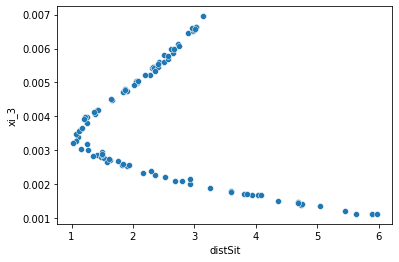
\includegraphics[width=\linewidth]{./SingleParam/xi_3_1.png}
            \caption{Attempt 1}
            \label{singlexi:1}
            \end{subfigure}
            \begin{subfigure}{.3\textwidth}
            \centering
            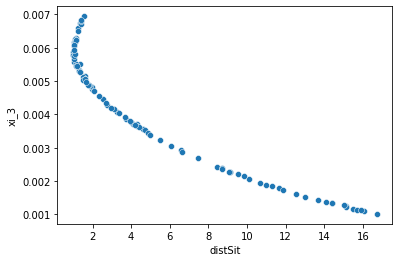
\includegraphics[width=\linewidth]{./SingleParam/xi_3_2.png}
            \caption{Attempt 2}
            \label{singlexi:2}
            \end{subfigure}
            \begin{subfigure}{.3\textwidth}
                \centering
                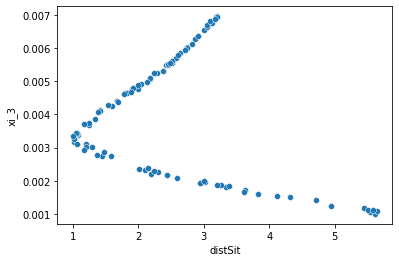
\includegraphics[width=\linewidth]{./SingleParam/xi_3_3.png}
                \caption{Attempt 3}
                \label{singlexi:3}
            \end{subfigure}
            
            \centering
            \begin{subfigure}{.3\textwidth} 
                \centering
                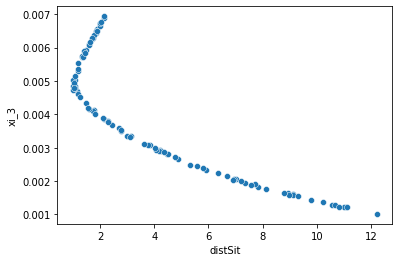
\includegraphics[width=\linewidth]{./SingleParam/xi_3_4.png}
                \caption{Attempt 4}
                \label{singlexi:4}
            \end{subfigure}
            \begin{subfigure}{.3\textwidth}
                \centering
                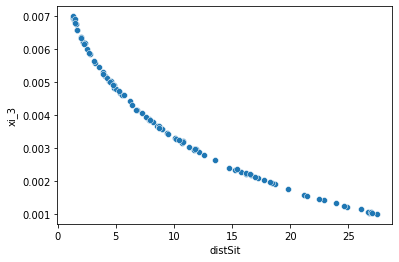
\includegraphics[width=\linewidth]{./SingleParam/xi_3_5.png}
                \caption{Attempt 5}
                \label{singlexi:5}
            \end{subfigure}

            \caption{$\xi_3$ values plotted against corresponding normalised Euclidean Distance between simulation and data means for 5 attempts.}
            \label{singlexi}
        \end{figure}


        For $\xi_3$ Grando's estimate was 0.0027. From our results we can deduce the following:
        \begin{itemize}
            \item Both \ref{singlexi:1} and \ref{singlexi:3} suggest the true value is around 0.003. 
            \item \ref{singlexi:2} and \ref{singlexi:4} suggest the true value is between 0.005 and 0.006.
            \item The negative gradient of \ref{singlexi:5} suggests the true value larger than our upper limit of 0.007.
        \end{itemize}
        Although it seems the value remains within the interval most of the time, it does not remain consistent. Again, as with $\lambda_3$, these changes in estimated value suggest the actual value may be changing through new attempts.







        \begin{figure}
            \begin{subfigure}{.3\textwidth}
            \centering
            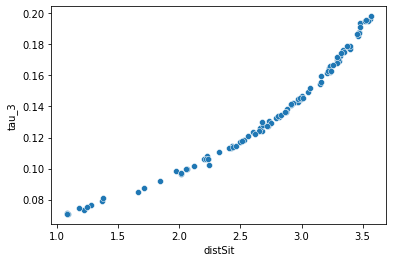
\includegraphics[width=\linewidth]{./SingleParam/tau_3_1.png}
            \caption{Attempt 1}
            \label{singletau:1}
            \end{subfigure}
            \begin{subfigure}{.3\textwidth}
            \centering
            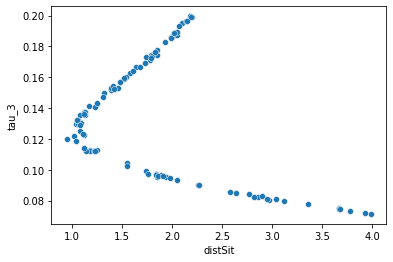
\includegraphics[width=\linewidth]{./SingleParam/tau_3_2.png}
            \caption{Attempt 2}
            \label{singletau:2}
            \end{subfigure}
            \begin{subfigure}{.3\textwidth}
                \centering
                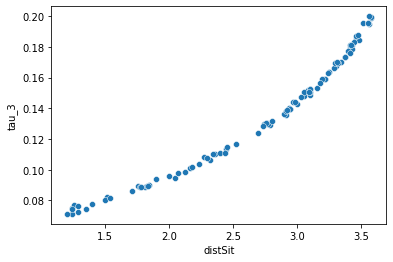
\includegraphics[width=\linewidth]{./SingleParam/tau_3_3.png}
                \caption{Attempt 3}
                \label{singletau:3}
            \end{subfigure}

            \centering
            \begin{subfigure}{.3\textwidth} 
                \centering
                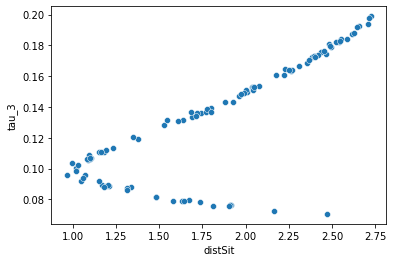
\includegraphics[width=\linewidth]{./SingleParam/tau_3_4.png}
                \caption{Attempt 4}
                \label{singletau:4}
            \end{subfigure}
            \begin{subfigure}{.3\textwidth}
                \centering
                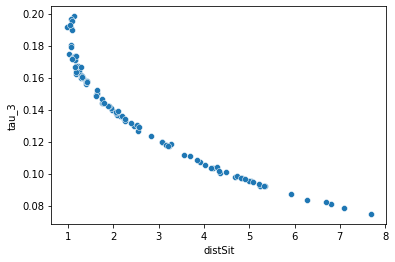
\includegraphics[width=\linewidth]{./SingleParam/tau_3_5.png}
                \caption{Attempt 5}
                \label{singletau:5}
            \end{subfigure}

            \caption{$\tau_3$ values plotted against corresponding normalised Euclidean Distance between simulation and data means for 5 attempts.}
            \label{singletau}
        \end{figure}


        For $\tau_3$ Grando's estimate was 0.0386. From our results we can deduce the following:
        \begin{itemize}
            \item The positive slope of \ref{singletau:1} and \ref{singletau:3} suggest the true value is below our lower bound of 0.07.
            \item \ref{singletau:2} suggests the true value is around 0.13.
            \item \ref{singletau:4} suggests the true value is around 0.10.
            \item The negative slope of \ref{singletau:5} suggests the true value is above our upper limit of 0.2.
        \end{itemize}
        Once again, multiple attempts provide contradicting results. This suggests the actual value is changing with each attempt.

        \subsubsection{Adjusted Algorithm}
        \label{Replicating_Existing_Rainfall_Model:Replicating_Grando:Results:Adjusted_Algorithm}

        From all \ref{singlelam}, \ref{singletau} and \ref{singlexi} we have the same indication; the parameter values are changing for new attempts. To justify this, we must isolate the cause of this change. Our model requires our nine parameters to be constants. Furthermore, we have controlled the values of each in our testing. Thus any change in parameter value must be caused by external factors. The only other factors within the model are the hidden Markov parameters. 

        Looking closely at our simulation algorithm, one may notice for each attempt, the HMM parameters are generated by a uniform random variable and then kept the same for each simulation. In other words, they only change on new attempts. When we estimate the parameters using ABC, we are conditioning the values of the parameters we have preset, particularly the HMM parameters. Since these vary for each attempt, the condition for our algorithm varies for each attempt. Thus, we can confirm the model is different for each attempt, and the parameters estimates are, in fact, also different for each attempt. 
        We can conclude ABC, with the given algorithm, has failed to provide parameter estimates. The increase in efficiency of the ABC algorithm has allowed for multiple attempts, highlighting a flaw in the algorithm itself. 

        We can further highlight this issue through an adjustment to the ABC algorithm. We move the generation of HMM parameters within the iterative process. This forces a new set of HMM parameters for each simulation. Whilst this would not be accurate to the model, this randomisation prevents the method by providing parameter estimates that fit a particular set of HMM parameters. We use this for three-parameter estimation. We increase the number of iterations to 1000 to ensure we can find a pattern if there is one as there is an increase in randomisation. Using the same parameter values as \ref{Replicating_Existing_Rainfall_Model:Replicating_Grando:Results:Three_Parameter_Estimation}, computation on the personal desktop took 652.842 seconds.

        \begin{figure}
            \begin{subfigure}{.3\textwidth}
            \centering
            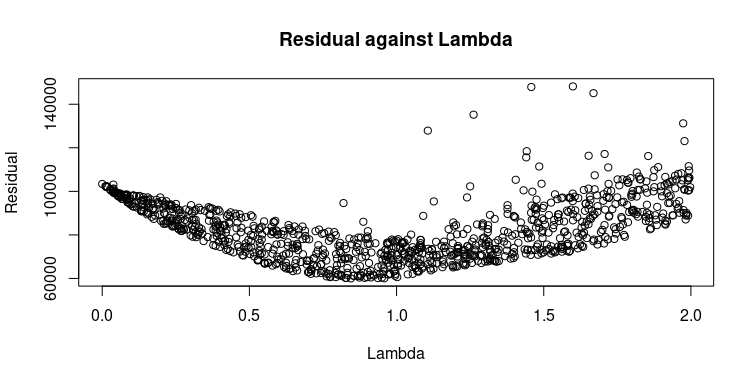
\includegraphics[width=\linewidth]{./Adj_ABC/lam_3.png}
            \caption{$\lambda_3$}
            \label{adj:1}
            \end{subfigure}
            \begin{subfigure}{.3\textwidth}
            \centering
            \includegraphics[width=\linewidth]{./Adj_ABC/xi_3.png}
            \caption{$\xi_3$}
            \label{adj:2}
            \end{subfigure}
            \begin{subfigure}{.3\textwidth}
                \centering
                \includegraphics[width=\linewidth]{./Adj_ABC/tau_3.png}
                \caption{$\tau_3$}
                \label{adj:3}
            \end{subfigure}

            \caption{Parameter values plotted against corresponding normalised Euclidean Distance between simulation and data means for simulation calculated using adjusted ABC algorithm}
            \label{adj}
        \end{figure}


        As we can see from Figures \ref{adj}, we have a somewhat uniform scatter. This result suggests we cannot find a parameter estimate for our non-HMM parameters without fixing the HMM parameters. Thus we must search for an alternative method of parameter estimation. Our method must support high-dimensional parameter estimation in our current model; we have 21 unknowns.
        




